% !TEX TS-program = pdflatex
% !TEX root = ../LightMicroRep.tex

%************************************************
\chapter{Ca-Imaging}
\label{chp:Ca-Imaging}
%************************************************

%----------------------------------------------------------------------------------------
%	INTRODUCTION
%----------------------------------------------------------------------------------------

\section{Introduction}

\paragraph{Aim} To obtain/depict changes in Calcium concentration of a blowfly salivary gland upon stimulation by serotonin.
\\

The blowfly salivary glands provide an ideal object for studying stimulus-dependent spatiotemporal intra- and intercellular Ca$^{2+}$ dynamics in an intact 'mini-organ', since its tubular secretory region is easily accessible to experimental manipulation and Ca$^{2+}$-imaging experiments. 
The secretory portion of the gland consists of a single layer of uniformly differentiated epithelial cells that are grouped around a central lumen \cite{Zimmermann1997}.
The membrane of a blowfly's salivary gland is covered by ion pumps. 
Due to the deep infoldings (canaliculi) of the apical membrane, there is a huge amount of ion pumps. These infoldings enlarges the apical membrane up to 250 times in comparison to a flat membrane. 
Normally, after dissection, the salivary gland produces almost no saliva. 
However, the presence of serotonin (5-HT) induces salivation. Serotonin itself has 2 different receptors on the plasma membrane. 

The detection of Ca$^{2+}$ utilizes the fluorescent dye fura 2 whose fluorescence emission is independent of Ca, but its excitation changes depending on [Ca$^{2+}$]. 
Fig.~\ref{fig:fura2} describes the excitation response of fura 2 due to Ca ions. 
The excitation maximum at nominally free Ca condition is at 365 nm (isosbestic point). However, the at high concentration of Ca, the excitation maximum sits at 340 nm. 
In contrast, the excitation at 380 nm decreases. 

\begin{figure}[h]
\centering
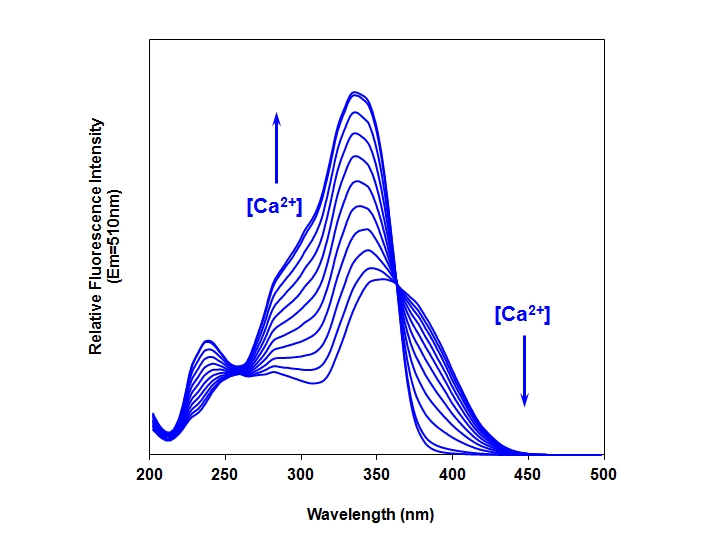
\includegraphics[width=.5\columnwidth]{Exp_8_CaImaging/Figures/fura2aatbio2}
\caption{Excitation spectrum of fura 2 fluorescent dye in the presence of Calcium. 
Image source: \href{https://www.aatbio.com/products/fura-2-am-ultrapure-grade-cas-108964-32-5}{\textit{https://www.aatbio.com/products/fura-2-am-ultrapure-grade-cas-108964-32-5}}. 
Accessed: 09/12/2020.} 
\label{fig:fura2}
\end{figure}

Since fluorescence intensity depends on the concentration of fluorophores, which in turn depends on cell conditions (bleaching, unequal distributions, volume changes, etc), measuring both excitation wavelength allows the elimination of these influencing factors and the signal then depends only on the concentration of calcium.

%----------------------------------------------------------------------------------------
%	METHODS
%----------------------------------------------------------------------------------------

\section{Methods}

The specimen is a dissected abdominal part of the salivary gland of \textit{Calliphora vicina}. 
The specimen is then loaded with the modified fluorescent dye fura 2. 

The imaging is conducted using an inverted microscope equipped with Fluar 20$\times$ 0.75 NA, a fluorite optic with high trasmission for UV light. 
The sample is then excited at 340 $\pm$ 5 nm and 380 $\pm$ 5 nm. 
Emission is filtered using a bandpass at 510 $\pm$ 42 nm. 
The light source a Xenon arc lamp that emits a white light with an even spectrum in the UV range. 
Wavelength selection for excitation is performed by a grating monochromator that passes a select wavelength through a slit.  

The gland was tested with different Serotonin (5-HT) concentrations (1, 3, and 10 nM). 
The reagents added is listed in Table~\ref{tab:seroca} along with the order and time of addition.

\begin{table}[hbt]
\caption{List of reagents}
\centering
\begin{tabular}{ccc}
\toprule
Reagent & Addition time \\
\midrule
Ringer				&start\\
1 nM 5-HT			&1 min\\
3 nM 5-HT 			&4 min\\
10 nM 5-HT 		&9 min\\
Normalringer 		&13 min\\
20 nM MnCl$_2$ 	&16 min\\
\bottomrule
\end{tabular}
\label{tab:seroca}
\end{table}

At the end of the measurement, $MnCl_2$ is added to quench the remaining fluorescence from Ca binded fura 2 and allows the requisition of autofluorescence from the sample itself. 
Substracting all the acquired measurement results by this background signal gives the actual fluorescence signal due to Ca.

%----------------------------------------------------------------------------------------
%	RESULTS AND DISCUSSION
%----------------------------------------------------------------------------------------
\section{Results and Discussion}

\begin{figure}[ht]
\centering
\subfloat[Excitation spectrum\label{exspec}]{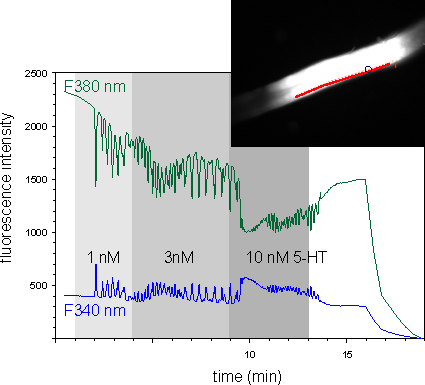
\includegraphics[width=.45\columnwidth]{Exp_8_CaImaging/Figures/drawing}} \hfil
\subfloat[Ratio of excitation spectrum\label{ratexspec}]{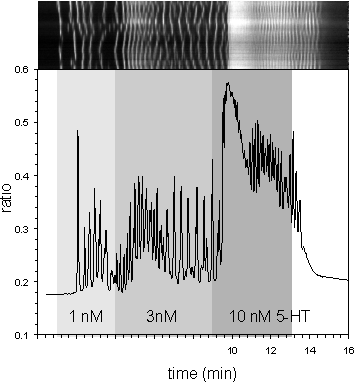
\includegraphics[width=.38\columnwidth]{Exp_8_CaImaging/Figures/drawing-1}}
\caption{Measurement results. \textbf{A} is the measurement result of the excitation spectra at 340 and 380 nm over time, inset is the selected region of interest on the specimen (red line with width 1 pixel.), \textbf{B} is ratio of the obtained spectra over time, inset is the space-time plot of calcium concentration. 
The addition of serotonin (5-HT) is marked on both figures accordingly.} 
\label{fig:CaIm}
\end{figure}

Observing the measurement result in Fig.~\ref{exspec}, it can be seen that there is an oscillation in the fluorescence signal obtained by stimulation of 5-HT under the concentration of 10 nM. 
This oscillation that is evident on one excitation spectrum (e.g. 340 nm) is mirrored on the other excitation spectrum (380 nm). 
The fluorescence oscillation increased even more after the addition of 10 nM 5-HT, which however in this experiment seemed like a plateau, the frequency incerease can only be observed minimally. 
Then afterwards the fluorescence signal decreases after quenching.

Indicators are charged molecules and do not easily pass lipid membranes. 
To promote the introduction of fluorescent indicators into the interior of single cells or tissue, the method that can be used is adding lipophilic groups (acetoxymethyl or acetate ester groups) to the charged indicator molecule. 
The indicator complex becomes neutral and lipophilic and hence membrane-permeant. 
Once the complex has entered into the cytosol, cytoplasmic esterases gradually cut off the lipophilic groups and the free indicator molecule is then trapped in the cytosol and ready to bind with Ca$^{2+}$ \cite{Islam2012}. 
However, if the concentration of fura 2 is too high, then there is the danger of influencing the physiology of the cell by the increase in concentration of the cut off lipophilic groups (acetic acid and formaldehyde)

The use of fura 2, a ratioing dye, in principle allows the quantitative determination of [Ca$^{2+}$]. 
This follows the Grynkiewicz equation (\ref{eq:Gr}).

\begin{equation}
 [Ca^{2+}] = K_{d} \times b \times \frac{R-R_{min}}{R_{max}-R} = K_{d}^{*} \times \frac{R-R_{min}}{R_{max}-R}\label{eq:Gr}
\end{equation}

$K_{d}$ is the dissociation constant of Ca, b is the instrument factor, $R_{max}$ is R at high [Ca$^{2+}$] (or saturating conditions), $R_{min}$ is R at [$Ca^{2+}$] = 0, R is the ratio of the measured fluorescence intensities, $K_{d}^{*}$ is the combination of b and $K_{d}$. 
The constant b along with $R_{min}$ and $R_{max}$ can be obtained by calibration. 
However the quantitative determination of [Ca$^{2+}$] was not performed in this experiment.

The red line in the inset of Fig.~\ref{exspec} shows the part where the fluorescence measurement was conducted. 
The obtained fluorescence ratio is presented in Fig.~\ref{ratexspec}. 
Here it can also be seen that by the addition of 1 nM 5-HT, oscillations can be observed. Oscillations of [Ca$^{2+}$] in response to intermediate agonist concentrations have been observed in many different cell. In the majority of non-excitable cells investigated so far, these oscillations are believed to be based on a periodic release of Ca$^{2+}$ from intracellular stores \cite{Zimmermann1997}. 
$Ca^{2+}$ in this experiment also exist extracellularly due to the Ringer solution which contains $CaCl_2$. 
The oscillation frequency increases by adding a higher concentration of Ca$^{2+}$ (5 nM). 
A jump in signal then occured after the addition of 10 nM 5-HT with an even higher frequency of oscillation. This fluorescence signal behaviour also coincides with the space-time plot provided as inset.

From Fig.~\ref{ratexspec}, it can be conclusively seen that serotonin (5-HT) induces the transport of Ca$^{2+}$ in blowfly salivary gland, which normally does not produce saliva after dissection. 
The concentration of Ca$^{2+}$ in blowfly salivary gland is responsive towards the amount of 5-HT that is added. 
 
%----------------------------------------------------------------------------------------
%	BIBLIOGRAPHY
%----------------------------------------------------------------------------------------

\renewcommand{\refname}{\spacedlowsmallcaps{References}} % For modifying the bibliography heading

%\bibliographystyle{unsrt}

%\bibliography{sample.bib} % The file containing the bibliography


